\documentclass[12pt, 
hyperref={colorlinks=true, linkcolor=blue, urlcolor=cyan}]{beamer}
\usetheme{default} 

\setbeamertemplate{navigation symbols}{} %gets rid of navigation symbols
\setbeamertemplate{footline}{} %gets rid of bottom navigation bars
\setbeamertemplate{footline}[page number]{} %use this for page numbers

\setbeamertemplate{footline}{%
  \raisebox{5pt}{\makebox[\paperwidth]{\hfill\makebox[10pt]{\scriptsize\insertframenumber~~}}}}

\setbeamertemplate{itemize items}[circle] %round bullet points
\setlength\parskip{10pt} % white space between paragraphs

\usepackage{wrapfig}
\usepackage{subfig}
\usepackage{setspace}
\usepackage{enumerate}
\usepackage{graphicx}
\usepackage{amsmath}
\usepackage{amsfonts}
\usepackage{amssymb}
\usepackage{amsthm}
\usepackage[UKenglish]{isodate}
\usepackage{tikz}
\usepackage{natbib}
\def\checkmark{\tikz\fill[scale=0.4](0,.35) -- (.25,0) -- (1,.7) -- (.25,.15) -- cycle;} 

% bracketing shortcuts
\newcommand{\paren}[1]{\left(#1\right)}
\newcommand{\sqbracket}[1]{\left[#1\right]}
\newcommand{\cbracket}[1]{\left\{#1\right\}}
\newcommand{\abs}[1]{\left\lvert#1\right\rvert}
\newcommand{\norm}[1]{\left\lVert#1\right\rVert}
% set up the argmin operator, argmax
\DeclareMathOperator*{\argmin}{arg\,min}
\DeclareMathOperator*{\argmax}{arg\,max}

\newcommand{\myframe}[1]{\begin{frame} \frametitle{#1}}
% the preamble
\title{Running GUI-less: an introduction}
\author{Brian Williamson}
\institute{BIOST 561: Computational Skills For Biostatistics I}
\date{10 November 2016}

% Start the document
\begin{document}
% The title page
\begin{frame}
\titlepage
\end{frame}

\myframe{Running GUI-less}
\begin{columns}[c]
\begin{column}{.66\textwidth}

\emph{GUIs are picture books --- they let you move things to other things, or right click on things and select options.

But you still type a post when you want to ask a question.

Command lines are much the same thing... if what you're trying to do is simple, then pictures and words are about the same. If what you're trying to do is complex, then words allow you to explain better.}

\vspace{2cm}
\href{http://unix.stackexchange.com/users/65333/sobrique}{Stack Exchange user} \texttt{Sobrique} (2015)
\end{column}
\begin{column}{.33\textwidth}

\includegraphics[width=1\textwidth]{sobrique.jpg}
\end{column}
\end{columns}
\end{frame}
% Motivation: typical R use, clusters are Linux
\begin{frame}[fragile]
\frametitle{Motivation}
A typical R learning curve (on a personal machine): 
\begin{enumerate}
\item Run commands by typing them line by line into a GUI (RStudio, RGUI, etc.), e.g.
\begin{verbatim}
> exp(1)
[1] 2.718282
> cos(pi)
[1] -1
> x <- 55
\end{verbatim}
\item[]
\item Use the GUI's editor (or e.g. Notepad++) to create scripts and save to use/edit/etc. later
\end{enumerate}

The first is actually the same as executing R from the command line, while the second is instrumental in writing long programs or simulation studies.
\end{frame}

\myframe{Motivation}
Why not keep running R using a GUI and (R) scripts?
\begin{itemize}
\item Requires keeping R/RStudio open while the script is running
\item[]
\item Can take up significant resources on a personal machine
\item[]
\item May need to open multiple R/RStudio windows to run multiple jobs (there are some ways around this)
\end{itemize}

Many courses (e.g. 570s) and research will require a more sophisticated approach.
\end{frame}

\section{Running GUI-less}
% introduce do.one, output, etc
\myframe{Example: permutation test}
Permutation tests construct a sampling distribution for a test statistic, like the bootstrap.

However, they are used for different things in inference: permutation test for hypothesis testing, bootstrap for confidence intervals (usually).

In permutation testing, we resample in a manner consistent with the \emph{null hypothesis}. These tests allow us to compute the sampling distribution for any test statistic (most useful when we do not actually know it), and obtain approximate p-values.
\end{frame}

\begin{frame}[fragile]
\frametitle{Example: permutation test}
Consider SNP data --- we want to measure difference in mean outcome in a dominant model for a single SNP. In this case, we could just use a $t$-test, but it is a nice illustration.

Some code to set this up:
\begin{verbatim}
## make up some data (thanks Ken!)
carrier <- rep(c(0,1), c(100,200))
## outcome under the null and alternative
null.y <- rnorm(300)
alt.y <- rnorm(300, mean = carrier/2)
\end{verbatim} 
\end{frame}

\begin{frame}[fragile]
\frametitle{Example: permutation test (more code)}
{\fontsize{10pt}{7.2}\selectfont
\begin{verbatim}
oneTest <- function(x, y) {
  ## get a new bootstrap sample of x
  xstar <- sample(x)
  
  ## return the difference in means
  ret <- mean(y[xstar == 1]) - mean(y[xstar == 0])
  
  return(ret)
}
## set a seed first!
set.seed(4747)
system.time(output.truenull <- replicate(10000, oneTest(carrier, 
            null.y)))
system.time(output.falsenull <- replicate(10000, oneTest(carrier, 
            alt.y)))
null.diff <- mean(null.y[carrier == 1]) - 
             mean(null.y[carrier == 0])
alt.diff <- mean(alt.y[carrier == 1]) - 
             mean(alt.y[carrier == 0])
\end{verbatim}
}

With 10000 replications, this takes approx. 2 seconds to run on Box
\end{frame}

% bootstrap vs permutation test
\myframe{Example: permutation test vs bootstrap ($H_0$ true)}
\begin{columns}
\begin{column}{.5\textwidth}
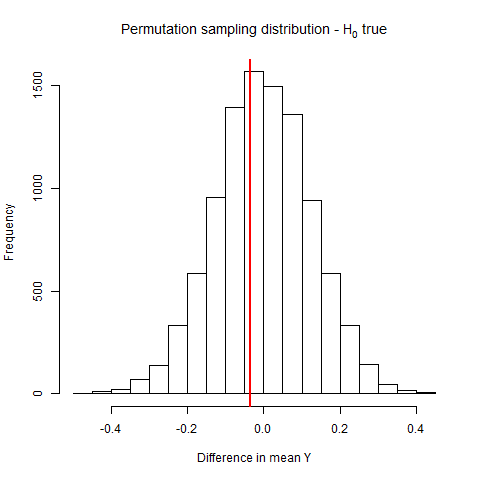
\includegraphics[width = 1\textwidth]{perm_true_null.png}
\end{column}
\begin{column}{.5\textwidth}
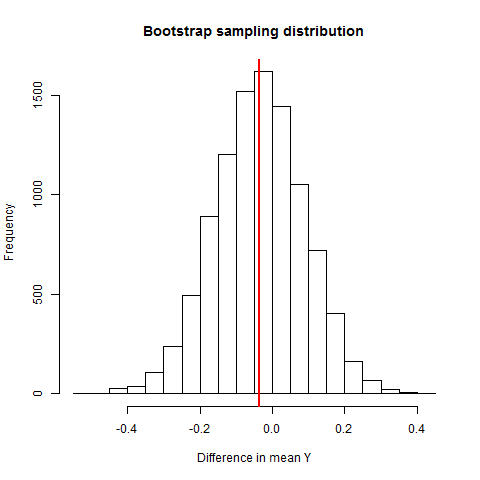
\includegraphics[width = 1\textwidth]{boot.png}
\end{column}
\end{columns}
$p$-value (computed as proportion greater than test statistic in original data) $\approx 0.77$
\end{frame}

\myframe{Example: permutation test vs bootstrap ($H_0$ false)}
\begin{columns}
\begin{column}{.5\textwidth}
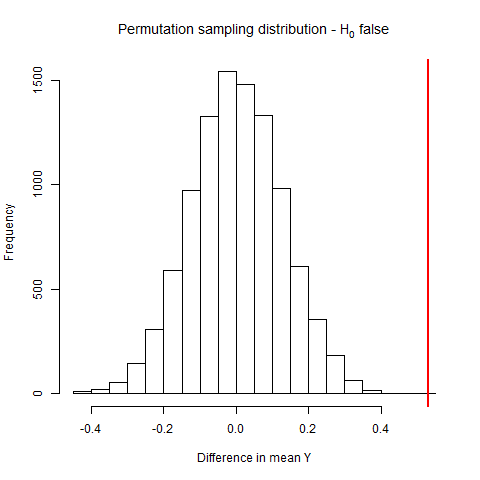
\includegraphics[width = 1\textwidth]{perm_false_null.png}
\end{column}
\begin{column}{.5\textwidth}
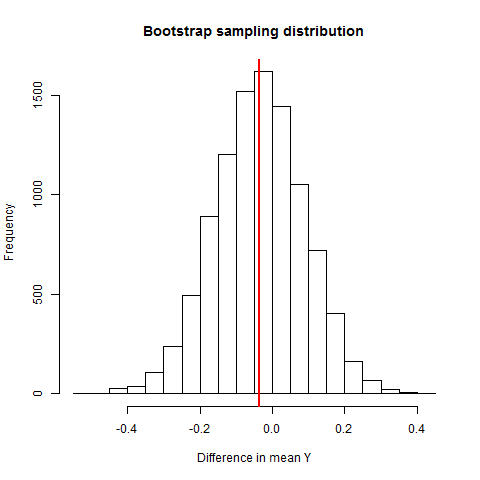
\includegraphics[width = 1\textwidth]{boot.png}
\end{column}
\end{columns}
$p$-value (computed as proportion greater than test statistic in original data) $< 0.005$
\end{frame}

% Running R from the command line: Rscript, saving values, setting seed, etc.
\myframe{Running GUI-less}
Three basic things to remember:
\begin{itemize}
\item You have to set a seed! 
\begin{itemize}
\item Without using \texttt{set.seed()}, you will not be able to reproduce output if necessary; either you won't know where the random number generator started, or you will get the same output for each script
\end{itemize}
\item[]
\item R will not automatically save any objects created during the session --- you have to do this manually
\item[]
\item You have to tell the computer where to look for the executable file to run your code
\end{itemize}
Bottom line: \textbf{Set the seed in a logical, memorable way such that each script gets a different seed. Also, save output that you care about to memory.}
\end{frame}

\begin{frame}[fragile]
\frametitle{Running GUI-less: Rscript}
While there are a few ways to run R GUI-less, \texttt{Rscript.exe} is one of the most common.

First, include where \texttt{Rscript.exe} resides on your machine. On Box (and most machines), it is in \texttt{/usr/local/bin/Rscript}. Put \texttt{\#!/usr/local/bin/Rscript} at the top of your \texttt{.R} file so that the computer knows how to run the code.

The ``shebang'', \texttt{\#!}, is common in GUI-less programming. This type of statement at the top of a file tells the computer where to look to run the file (more on this in shell scripting).

\end{frame}

\begin{frame}[fragile]
\frametitle{Running GUI-less: running the script}
Doing this on Mac or Linux is easy --- simply navigate to the file and run it, e.g.{\tiny
\begin{verbatim}
cd "C:/Users/brianw26/Dropbox/Courses/2016-2017 Third Year/Presentations/BIOST 561 - Lecture"
Rscript permutation_test_example.R
\end{verbatim}
}
On Windows:
\begin{itemize}
\item Need to set the PATH (only once) to tell the machine where to look for \texttt{Rscript.exe}
\item Typing \texttt{path} in the command line brings up the PATH, typing
{\scriptsize \texttt{C:\textbackslash Program Files\textbackslash R\textbackslash R-3.2.1\textbackslash bin\textbackslash x64;\%PATH\%} } (or wherever your R install is) will add this to the PATH
\end{itemize}
Then run with 
{\tiny
\begin{verbatim}
cd "C:\Users\brianw26\Dropbox\Courses\2016-2017 Third Year\Presentations\BIOST 561 - Lecture"
Rscript permutation_test_example.R
\end{verbatim}
}
\end{frame}


\begin{frame}[fragile]
\frametitle{Running GUI-less: parameters}
In the permutation test example, we had three parameters: $n$ (sample size), $B$ (number of Monte Carlo replications), and the seed.

That is more clear in this function:
{\scriptsize
\begin{verbatim}
permTestSNP <- function(n = 300, B = 10000) {
carrier <- rep(c(0, 1), c(n/3, 2*n/3)) ## make the genotypes (0/1)
  null.y <- rnorm(n) ## make y under the null hypothesis
  alt.y <- rnorm(n, mean = carrier/2) ## make y under the alternative 
  output.truenull <- replicate(B, oneTest(carrier, null.y)) ## run the test B times
  output.falsenull <- replicate(B, oneTest(carrier, alt.y))
  ## get the observed difference in means
  null.diff <- mean(null.y[carrier == 1]) - mean(null.y[carrier == 0])
  alt.diff <- mean(alt.y[carrier == 1]) - mean(alt.y[carrier == 0])
  ## return the sampling distribution and the p-values
  return(list(samp.truenull = output.truenull, samp.falsenull = output.falsenull,
              p.truenull = mean(abs(output.truenull)) > abs(null.diff),
              p.falsenull = mean(abs(output.falsenull)) > abs(alt.diff))
         )
}
\end{verbatim}
}
\end{frame}

\begin{frame}[fragile]
\frametitle{Running GUI-less: setting the seed}
Rscript lets us pass arguments to our R session when we run a script.

However, we need a bit of pre-processing to read that in:
{\scriptsize
\begin{verbatim}
#!/usr/local/bin/Rscript
## read in the parameter(s)
arg <- commandArgs(TRUE)
## gets read in as a character, change to numeric
myseed <- as.numeric(arg)

permTest <- function(n = 300, B = 10000) {
 <code omitted, see earlier slides>
}
set.seed(myseed)
output <- permTest(n = 300, B = 10000)
\end{verbatim}
}

At the command line, enter e.g. \texttt{Rscript permTest.R 47} to run \texttt{permTest} with $n = 300$, $B = 10000$, and seed = 47.
\end{frame}

\begin{frame}[fragile]
\frametitle{Running GUI-less: setting multiple parameters}
Sometimes we have multiple parameters, e.g. $n$, $B$, and seed.

We can read in multiple from Rscript:
{\scriptsize
\begin{verbatim}
args <- commandArgs(TRUE)
if (length(args) == 0) {
  print("No arguments supplied.")
} else {
  for (i in 1:length(args)) {
    eval(parse(text = args[i]))
  }
}
if (!exists("myn")) {
  myn <- 100
  cat("Note: assuming n = 100")
}
if (!exists("myseed")) {
  myseed <- 47
  cat("Note: setting seed to be 47")
}
if (!exists("myB")) {
  myB <- 1000
  cat("Note: running 1000 replications")
}
\end{verbatim}
}
\end{frame}

\begin{frame}[fragile]
\frametitle{Running GUI-less: setting multiple parameters}
We then pass Rscript multiple parameters, e.g. \texttt{Rscript permTest.R myn=300 myseed=47 myB=10000}

The code on the previous slide makes sure that You can debug Your output.

Remember that \texttt{commandArgs()} reads in characters! This is a common source of error --- we don't want to make R angry.
\end{frame}

\myframe{Running GUI-less: saving output}
\texttt{write.table()} and \texttt{write.csv} are useful for large output datasets.

\texttt{save()} writes an R-friendly version of an object (or objects) to a designated \texttt{file}; read these in with \texttt{load()}.

``How much/what to save?'' --- depends on what you need!
\begin{itemize}
\item More output can make debugging easier, but wastes memory and/or time
\item Thinking through which output you want to save can make your results cleaner
\end{itemize}
\end{frame}

\begin{frame}[fragile]
\frametitle{Running GUI-less: saving output}
We might have, at the bottom of our script file, 
\begin{verbatim}
<...>
set.seed(myseed)
output <- permTest(n = myn, B = myB)
save(output, paste("perm_test_output_n_", myn, 
"_s_", myseed, "_B_", myB, ".Rdata", sep = ""))
\end{verbatim}

This creates a \texttt{.Rdata} file in the current working directory (where you called \texttt{Rscript} from), and is called e.g. \texttt{perm\_test\_output\_n\_300\_s\_47\_B\_10000.Rdata}
\end{frame}

\begin{frame}[fragile]
\frametitle{Running GUI-less: some advice}
Work up code slowly!
\begin{itemize}
\item Make sure your base code (e.g. \texttt{oneTest}) works correctly
\item Make sure the loop works (usually in GUI) (e.g. \texttt{permTest} with small B)
\item Make sure the looping and parameter setting works in Rscript, with small B (check output!)
\end{itemize}

Once your code passes all of these checks, \emph{then} run with a large B.
\end{frame}

\end{document}